%\documentclass[11pt, a4paper]{article}
\documentclass[includeheaders]{scrartcl}
\usepackage{scrlayer-scrpage}
\usepackage{hyperref}
\usepackage[utf8]{inputenc}
% Deutsche Silbentrennung
\usepackage[ngerman]{babel}
% Unterstützung für Farben
\usepackage[dvipsnames]{xcolor}
% Erweiterte Mathematik-Symbole
\usepackage{amsmath,amscd,amssymb}
% Nummerierte Listen
\usepackage{enumerate}
% Erweiterte Bildeinbettungsoptionen
\usepackage{graphicx}
% Typografisch hochwertige Tabellen
%\usepackage{tabularx,ragged2e,booktabs}
\usepackage{tabularx}
% Unterstützung für Unter-Abbildungen (z.B. 2x2-Matrix)
\usepackage{float}
\usepackage{caption}
\usepackage{subcaption}
% Seitenränder
\usepackage{geometry}
\geometry{a4paper,
	left=2.5cm,
	right=2.5cm,
	top=2.5cm,
	bottom=2.5cm}

% Unterstützung für °-Zeichen
\usepackage{textcomp}
\usepackage{gensymb}
% Formatierung von \paragraph und \subparagraph anpassen
\makeatletter
\renewcommand\paragraph{\@startsection{paragraph}{4}{\z@}%
	{-3.25ex\@plus -1ex \@minus -.2ex}%
	{1.5ex \@plus .2ex}%
	{\raggedsection\normalfont\sectfont\size@paragraph}%
}
\renewcommand\subparagraph{\@startsection{subparagraph}{5}{\z@}%
	{-3.25ex\@plus -1ex \@minus -.2ex}%
	{1.5ex \@plus .2ex}%
	{\raggedsection\normalfont\sectfont\size@subparagraph\mdseries}%
}
\makeatother
\usepackage{lastpage}
\setkomafont{pageheadfoot}{\sffamily} 
\sloppy
\parindent0mm
\parskip3mm

\addto\captionsenglish{% Replace "english" with the language you use
	\renewcommand{\contentsname}%
	{Inhaltsverzeichnis}%
	\renewcommand{\figurename}%
	{Abbildung}%
	\renewcommand{\tablename}%
	{Tabelle}%
}
\addto\captionsngerman{% Replace "english" with the language you use
	\renewcommand{\contentsname}%
	{Inhaltsverzeichnis}%
	\renewcommand{\figurename}%
	{Abbildung}%
	\renewcommand{\tablename}%
	{Tabelle}%
}

\begin{document}
% o - outer, i - inner, c - center -> location of header/footer-element
%\ohead{
\includegraphics[scale=0.5]{img/HPI-Logo.png}}
%\ifoot{
\includegraphics[scale=0.5]{img/HPI-Logo.png} }
\ifoot{
\includegraphics[scale=0.07]{img/logo}}
\cfoot{Template zur Veranstaltung Modellierung II, \\ Holger Giese, Sommersemester 2016}
\ofoot{\thepage}



\newpage 

\title{Analysedokument\\ \small{(Veranstaltung Modellierung II, SoSe 2016)}}
\date{}
\author{}

\maketitle
\begin{table}[H]
	\centering
	\begin{tabular}{lp{7.5cm}}
		\textbf{Projekt:} & Roboterbasiertes Personentransportsystem\\
		&\\
		\textbf{Auftraggeber: }& Prof. Holger Giese \newline Hasso-Platter-Institut \newline Prof.-Dr.-Helmert-Str. 2–3 \newline 14482 Potsdam\\
		&\\
		\textbf{Auftragnehmer: }& Modellierung II – Projektgruppe 5 \\
	\end{tabular}
\end{table}
 
\newpage

\begin{table}[H]
	\centering
	\begin{tabularx}{\textwidth}{|p{4cm}|X|p{4cm}|}
		\hline
		Verantwortlichkeit & Name, Vorname & Datum \\ \hline
		Ansprechpartner    & Bischoff, Sebastian & 06.06.2016 \\
		Bearbeitender      & Sauder, Jonathan & 06.06.2016 \\ 
		Bearbeitender      & Lüpke, Fabian & 06.06.2016 \\ 
		Bearbeitender      & Hering, Jonas & 06.06.2016 \\
		Bearbeitender      & Braun, Jakob & 06.06.2016  \\
		Bearbeitender      & Cremerius, Jonas & 06.06.2016 \\
		Bearbeitender      & Wischner, Jakob & 06.06.2016 \\
		Bearbeitender      & Schwenkert, Daniel & 06.06.2016 \\
		Bearbeitender      & Jäkel, Dominik & 06.06.2016 \\
		Bearbeitender      & König, Bastian & 06.06.2016 \\ \hline
	\end{tabularx}
\end{table}

\newpage

\tableofcontents

\newpage


\section{Zielbestimmung}
Die Aufgabe des Projektteams ist es ein System zu entwickeln, das selbstfahrende Roboter in einer Stadt der Zukunft koordiniert. Die Roboter werden für einen Krankentransportdienst eingesetzt. In dieser Stadt existieren keine Straßen mehr – umso komplexer wird die Steuerung der Roboter. Die größte Schwierigkeit stellt hier der Prozess, das Navigationsverhalten der Roboter mit den richtigen Parametern einzustellen und zu modellieren, dar. Ein weiterer Teil der komplexen Aufgabe besteht darin, die verschiedenen Krankentransporter in einer Weise zu synchronisieren, dass keine gegenseitigen Behinderungen auftreten. Die Voraussetzungen und Spezifikation dafür zu erfassen, ist Ziel dieser Analyse – die sich mit dem Fahr- und dem Aufladevorgang der Roboter, im speziellen den Fahrvorgang mit Patienten, ihren Manövrierfähigkeiten gegenüber Hindernissen, dem Aufnahmevorgang und die Entsendung zum Standort von Patienten beschäftigt.\\

Im weiteren Verlauf des Projektes könnten weitere Gegebenheiten auftreten, an die man das System anpassen müsste. Alle hier getroffenen Annahmen, Modellierungen und Implementierungen könnten damit im Rahmen der späteren Anwendungen revidiert werden.\\

Als Ausgangspunkt stellt das Unternehmen eine unbegrenzte Anzahl von Krankentransportrobotern zur Verfügung, die mit Aktoren, Sensoren und einem Ortungsgerät ausgestattet sind, und im Wechselspiel mit einem Server agieren.\\

Das Primärziel dieser Analyse ist es, dabei einen möglichst reibungslosen Ablauf der Krankentransporte für menschliche Individuen zu ermöglichen. Davon würde die Zielgruppe, spezifisch die Bewohner der Stadt, nachhaltig profitieren, indem Verkehrsunfällen, Staus und die Dauer des Fahrens auf ein Minimum reduziert werden – und somit Verletze stets rechtzeitig zur Behandlung im Krankenhaus eintreffen würden. Die Umsetzung des Systems birgt jedoch zahlreiche Herausforderungen, die im Verlauf dieser Analyse betrachtet werden. Falls die verschiedenen Hürden gemeistert werden, könnte langfristig ein einzelnes Unternehmen die gesamte Krankentransportinfrastruktur einer Großstadt übernehmen. Das System wird von sich aus selbstständig und vollständig autonom agieren. Unter Beachtung von Sicherheitsregeln, sollten damit keine weiteren Vorkenntnisse für Patienten und ihre Begleiter notwendig sein, um den Krankentransportdienst zu nutzen. Gerade für Patienten sollten die Roboter den Fahrvorgang allerdings mit kleinstmöglichem Aufwand und Belastung gestalten.\\\\

Definition des Problembereichs\\
Der Problembereich erweitert sich für diese Analyse auf sechs Punkte, um eine Gesamtkoordination effizient zu gestalten:\\

\begin{enumerate}
	\item Zuallererst muss das automatische Fahren im zweidimensionalen Koordinatensystem zu einem angegebenen Zielpunkt fehlerfrei möglich sein. Ebenfalls steht eine manuelle Steuerung zur Verfügung, um unerwarteten Ereignissen zu begegnen, die allerdings wiederum sinnvoll in das Gesamtsystem integriert werden muss.
	\item Als zweite Herausforderung gilt es einen möglichst reibungs- und unterbrechungslosen Batteriebetrieb zu garantieren, um zeitlich vorausschauendes Fahren zu ermöglichen. Im Falle eines niedrigen Batteriestands also unverzüglich an eine Ladestation anzudocken und aufzuladen, beziehungsweise längere Fahrten nicht anzutreten, für die der Batteriestand nicht ausreicht.
	\item Im dritten Punkt geht es darum den Schaden von Kollisionen zu minimieren; wie diese erkannt, wie auf sie reagiert wird und diese Kollisionen durch vorrauschendes Umfahren von Objekten verhindert werden können. Dies schließt sowohl bewegliche Objekte als auch unbewegliche Objekte mit ein. Im Speziellen muss eine Priorisierung der Roboter stattfinden, damit den Krankentransportern ein reibungsloser Fahrtverlauf garantiert wird.
	\item Dieser Punkt beschäftigt sich mit dem Abholvorgang. Jeder Krankentransport benötigt mindesten ein Vehikel das zur Verfügung steht. Jeder dieser Roboter muss unter bestimmten Kriterien wie Nähe und Batteriestand vom Server ausgewählt werden, und es gilt einzugrenzen, inwieweit diese Kriterien Einfluss auf die Entscheidung des Servers nehmen. Wenn dieser Roboter angekommen ist, müssen wiederum Patient und mögliche Helfende benachrichtigt werden.
	\item Außerdem muss das Fahrverhalten an einen Transport mit Patienten angepasst werden. Welche Daten werden ausgetauscht, damit dem Patienten nach der Ankunft die schnellstmögliche Behandlung zukommen kann?
\end{enumerate}

An die Punkte anknüpfend wird mit folgenden Annahmen gearbeitet:\\
\begin{enumerate}
	\item Zur Vereinfachung des Fahrverhalten muss jedes Zielobjekt physisch erreichbar sein. Ziele sind dementsprechend keine Hindernisse, das gleiche gilt für Ladestationen.
	\item Roboter können autark vom Server agieren, damit ihre Ziele bestimmen und eine Ladestation anfahren.
	\item Bei den beweglichen Objekten wird davon ausgegangen, dass es sich im Verkehrsbetrieb ausschließlich um andere Roboter handelt. Für die unbeweglichen Objekte ist es notwendig, dass ihre Position von vornerein bekannt ist und sie unverändert bleibt.
\end{enumerate}

\pagebreak



	\section{Produkteinsatz}
	
	\subsection{Beschreibung des Problembereichs}
	Im folgenden wird der wesentliche Problembereich um eine effiziente, reibungslose, und sichere Gesamtkoordination zu erreichen beschrieben.\\

Zuallererst muss das automatische Fahren im zweidimensionalen Koordinatensystem zu einem angegebenen Zielpunkt fehlerfrei möglich sein. 
	Die autonome Steuerung des Roboters muss in der Lage sein, unerwarteten Ereignissen und Hindernissen zu begegnen und diese erfolgreich und unfallfrei zu umfahren. Hindernisse können dabei statisch oder beweglich sein.\\
	
Als zweite Herausforderung gilt es einen möglichst reibungs- und unterbrechungslosen Batteriebetrieb zu garantieren, um zeitlich vorausschauendes Fahren zu ermöglichen. Im Falle eines niedrigen Batteriestands muss also unverzüglich eine Ladestation angefahren werden um aufzuladen. Außerdem sollen längere Fahrten nicht von Robotern entgegengenommen werden können, deren Akkustand nicht ausreicht um diese Fahrt ergolgreich zu absolvieren.\\

Im dritten Punkt geht es darum, einen Ablauf zu modellieren, für den unglücklichen Fall, dass ein Roboter kaputt gehen sollte. Dies könnte zum Beispiel in einem Unfall passieren.\\

Taxikunden können über eine Serviceapp Anfragen an das System schicken. Das System verwaltet eine Warteschlange, in die neue Aufträge aufgenommen werden. Andererseits können Kunden jederzeit ihre Anfrage abbrechen. Der Server muss die Aufträge in der Warteschlange effizient verteilen, im Speziellen muss eine Priorisierung der Roboter stattfinden, damit jedem Krankentransporter vor dem Taxiservice ein reibungsloser Fahrtverlauf garantiert wird.\\

Die Roboter müssen unter bestimmten Kriterien wie Nähe zum Ziel und aktuellem Batteriestand vom Server ausgewählt werden, und es gilt einzugrenzen, inwieweit die Kriterien wiederum Einfluss auf die Entscheidung des Servers nehmen.\\

Wenn ein Roboter bei einem Patienten oder einem Kunden angekommen ist, müssen Patient und mögliche Helfende bzw. der Fahrtgast benachrichtigt werden. Außerdem muss das Fahrverhalten bzw. die Geschwindigkeit an einen Transport mit Patienten angepasst werden.\\

An die Punkte anknüpfend wird mit folgenden Annahmen gearbeitet:
\begin{enumerate}
	\item Wir starten das System mit voll geladenen Akkus für jeden Roboter
	\item Es existiert genau ein Hospital
	\item Die Kommunikation funktioniert zuverlässig, insbesondere kommen alle gesendeten \textit{Messages} auch bei dem Empfänger ungeschädigt an. Dazu nehmen wir auch an, dass die Latenz vernachlässigbar klein ist.
	\item Zur Vereinfachung des Fahrverhalten muss jedes Zielobjekt physisch erreichbar sein. Ziele sind dementsprechend keine Hindernisse, das Gleiche gilt für Ladestationen, und sind prinzipiell mit einer Akkuladung erreichbar.
	\item Der Batterieverbrauch bei Robotern ist in einem linearen Verhältnis zur zurückgelegten Strecke.
	\item Bei den beweglichen Objekten wird davon ausgegangen, dass es sich im Verkehrsbetrieb ausschließlich um andere Roboter handelt. 
	Für die unbeweglichen Objekte ist es notwendig, dass ihre Position unveränderlich ist.
	\item Im Falle, dass ein Roboter kaputt geht, wird dieser nach einer endlichen Zeit von einem externen, nicht modellierten Unternehmen repariert und kann von seiner letzten Position aus wieder fahren.
	\item Ein Patient ist immer von Helfenden umgeben, die ermöglichen, dass der Patient auf den Roboter geladen wird, und nach der Verladung diesbezüglich das Krankenhaus benachrichtigen.
	\item Wenn ein Kunde ein Taxi bestellt und dieses ankommt, steigt dieser auch zeitnah ein und nimmt seine Fahrt wahr.
	\item Der Taxikunde schließt nach Ankunft bei seinem Ziel die Taxifahrt ab. Er schickt über die TaxiApp also eine entsprechende Nachricht an das System.
	\item Aufträge vom Krankenhaus kommen zunächst auf die vom Server verwaltete Warteliste und erhalten die Wartelisteposition als Nachricht. Wenn das Krankenhaus diese Wartelisteposition nicht passt, kann der Auftrag analog zum Taxiauftrag zurückgezogen werden.

\end{enumerate}

\pagebreak

		\subsection{Glossar}

		% \begin{description}
		% 	\item[Robot]{Roboter, der sich im 2-Dimensionalen Raum bewegen kann.}
		% 	\item[Server]{Verteilt Aufträge an die Roboter}
		% 	\item[Charger]{Ladestation für den Roboter}
		% 	\item[Destination]{Vom Server verwaltete Ziele, die der Roboter ansteuern kann.}
		% 	\item[Obstacle]{Hindernisse, die der Roboter erkennt und umfährt.}
		% \end{description}

			\begin{tabular}{ l p{10cm} }
		\textbf{Begriff} & \textbf{Erklärung}\\
		Robot & Roboter, der sich im 2-Dimensionalen Raum bewegen kann. Der wird
		als Fahrzeug verwendet und kann Personen transportieren.\\
		Position & Eine Position ist eine Zweidimmensionale Position im Raum,
		also ein Punkt, zu dem der Roboter fahren kann\\
		Task & Ein Task behinhaltet zusätzlich zu einer Position auch eine
		Geschwindigkeit. Fadurch kann der Server dem Roboter mitteilen, ob
		dieser vorsichtig oder schnell zu einer Position fahren
		soll.\\
		Server & Der serve ist eine einzelne, zentrale Instanz, die die Aufträge
		an die Roboter verteilt\\
		Charger & Ladestation für den Roboter\\
		Destination & Ziele die der Roboter ansteuern kann.\\
		Obstacle & Hindernisse, die der Roboter erkennt und umfährt Dies können
		entweder andere Roboter sein, mit denen der Roboter kommunizieren kann
		um eine Priorität festzulegen oder statische Hindernisse der
		Umgebung.\\
		Hospital & Das Krankenhaus, das mit dem System kommuniziert, um die Robots
		für Krankentransporte einzusetzen.
	\end{tabular}

		
		
		\subsection{Modell des Problembereichs}
		Abbildung \ref{fig:2-3-modell-problembereich} zeigt ein Klassendiagramm, welches das Modell des Problembereichs grafisch darstellt.
		\begin{figure}[H]
			\centering
			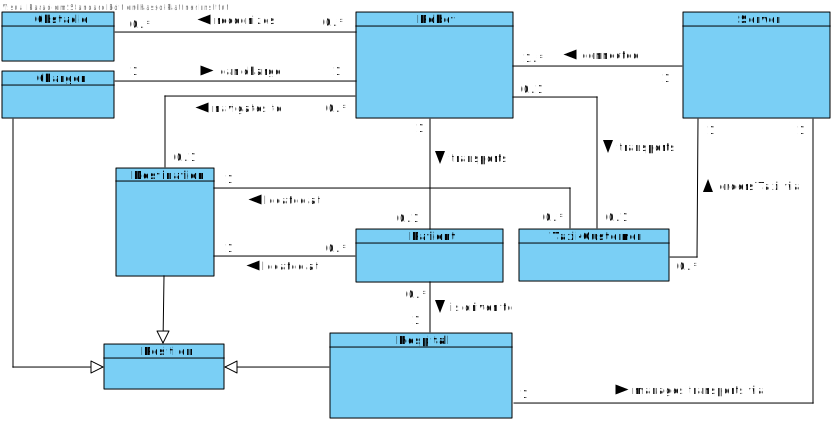
\includegraphics[width=0.8\textwidth]{img/1-Analyse-2}
			\caption{Klassendiagramm des Problembereichs}
			\label{fig:2-3-modell-problembereich}
		\end{figure}

		\subsection{Beschreibung der Geschäftsprozesse}

			\subsubsection{Beschreibung zu 1: Choose Robot}

			\begin{table}[H]
				\centering
				\begin{tabularx}{\textwidth}{|p{3cm}|X|}
				\hline
				\textbf{Auslösendes Ereignis:} & Der Server will den für ein bestimmtes Ziel bestmöglichen Roboter auswählen und diesen zum Ziel schicken. \\ \hline
				\textbf{Ergebnis:} & Alle Roboter haben ihre Sensordaten ausgelesen und diese dem Server
				mitgeteilt. 
				Daraufhin hat der Server einen Roboter ausgewählt, der für
				die Zielanfahrung optimal geeignet ist, und diesem den Auftrag zum
				Anfahren des Ziels übermittelt. \\ \hline
				\textbf{Mitwirkende:} &	Server, Roboter \\
				\hline
				\end{tabularx}
				\label{tab:2-4-choose-robot}
			\end{table}

			Abbildung \ref{fig:2-4-choose-robot-aktivitaetendiagramm} zeigt ein Aktivitätendiagramm, welches den Ablauf des Geschäftsprozesses \emph{1: Choose Robot} darstellt.
			\begin{figure}[H]
				\centering
				\includegraphics[width=\textwidth]{img/1-Analyse-3-Choose_Robot}
				\caption{Illustration von \emph{1: Choose Robot} durch Aktivitätendiagramm}
				\label{fig:2-4-choose-robot-aktivitaetendiagramm}
			\end{figure}

			Um den für ein gegebenes Ziel bestmöglichen \emph{Robot} auszuwählen, sendet
			der \emph{Server} zunächst an alle \emph{Robots} eine Anfrage (\emph{request}),
			woraufhin die \emph{Robots} ihre Sensordaten (\emph{sensor data}) auslesen und
			an den \emph{Server} senden. Auf Grundlage dieser Daten wählt der \emph{Server} den
			\emph{Robot} aus, der für die Erfüllung des Zieles am besten geeignet ist. 
			Es kann auch vorkommen, dass kein \emph{Robot} geeignet ist, um ein Ziel zu erfüllen. 
			Wie die Sensordaten und der Algorithmus zur Wahl des optimalen \emph{Robots} konkret definiert sind, ist eine Entwurfsentscheidung.

			\subsubsection{Beschreibung zu 2: Drive to Destination}

			\begin{table}[H]
				\centering
				\begin{tabularx}{\textwidth}{|p{3cm}|X|}
				\hline
				\textbf{Auslösendes Ereignis:} & Ein \emph{Robot} hat eine \emph{Destination} erhalten.\\ \hline
				\textbf{Ergebnis:} & Der \emph{Robot} ist unter Umfahrung von womöglichen \emph{Obstacles} zur \emph{Destination} gefahren.\\ \hline
				\textbf{Mitwirkende:} &	Ein einzelner, autonomer \emph{Robot}. \\
				\hline
				\end{tabularx}
				\label{tab:2-4-drive-to-destination}
			\end{table}
			
			\emph{Aufgrund des in der Analyse nicht näher spezifizierten Ablaufs von \emph{Drive to Destination} 
			entfällt hier ein Aktivitätendiagramm.}

			Dieser Prozess wird autonom vom \emph{Robot} ausgeführt. 
			Er wird genau dann ausgeführt, wenn der Roboter einen \emph{Task} vom Server erhalten hat, den er erfüllen soll. 
			Dabei wird vorher festgelegt, mit welcher Geschwindigkeit der \emph{Robot} die in dem \texttt{Task} enthaltene(n) \emph{Destination(s)} jeweils anfahren soll. 
			Damit können bei einem Auftrag vom \emph{Hospital} Patienten schnell erreicht werden und sicher zur Klinik gebracht werden. 
			Da der \emph{Robot} an dieser Stelle dem Server schon bestätigt hat, dass sein Akkustand für die Ausführung des \emph{Tasks} ausreichend ist, 
			ist der einzige Sonderfall, den wir betrachten müssen, dass ein \emph{Obstacle} auf der direkten Linie zwischen \emph{Robot} und \emph{Destination} liegt. 
			Dann wird der \emph{Robot} nach Wahl des besten Umweges das \emph{Obstacle} umfahren und wieder die Fahrt zur \emph{Destination} aufnehmen.

			\subsubsection{Beschreibung zu 3: Distribute Order}

			\begin{table}[H]
				\centering
				\begin{tabularx}{\textwidth}{|p{3cm}|X|}
				\hline
				\textbf{Auslösendes Ereignis:} & Ein \emph{User} hat eine neue \emph{Order}, die von dem System bearbeitet werden soll.\\ \hline
				\textbf{Ergebnis:} & Die \emph{Order} wird im System aufgenommen und entweder sofort oder sobald ein \emph{Robot} bereit ist bearbeitet.\\ \hline
				\textbf{Mitwirkende:} &	Ein \emph{User} und der \emph{Server}. \\
				\hline
				\end{tabularx}
				\label{tab:2-4-distribute Order}
			\end{table}

			Abbildung \ref{fig:2-4-distribute-order-aktivitaetendiagramm} zeigt ein Aktivitätendiagramm, welches den Ablauf des Geschäftsprozesses \emph{3: Distribute Order} darstellt.

			Ein \emph{User} hat eine \emph{Order}, die das System bearbeiten soll. Diese \emph{Order} wird dem \emph{Server} mitgeteilt, woraufhin der \emph{Server} einen neuen \emph{Task} erstellt. Dieser wird je nach Verfügbarkeit der \emph{Robots} und Priorität des \emph{Tasks} an einen \emph{Robot} verteilt, oder in die vom \emph{Server} verwaltete Warteliste aufgenommen. Der \emph{User} kann über den Use-Case \texttt{Cancel Order} seine \emph{Order} jederzeit während der Ausführung dieses Geschäftsprozesses zurückziehen.
			
			\begin{figure}[H]
				\centering
				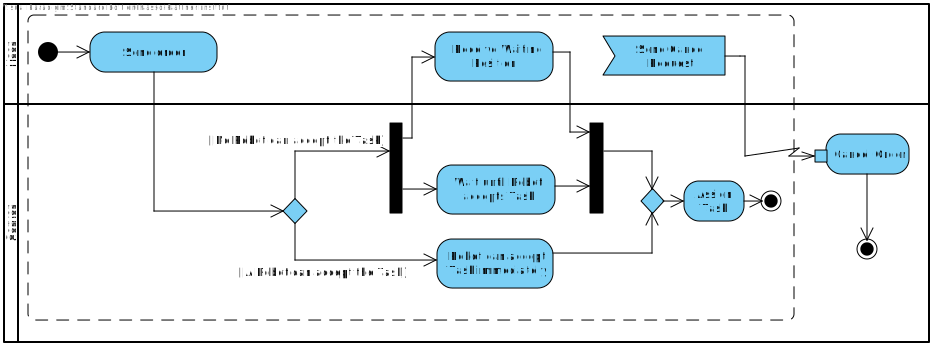
\includegraphics[width=\textwidth]{img/DistributeOrder}
				\caption{Illustration von \emph{3: Distribute Order} durch Aktivitätendiagramm}
				\label{fig:2-4-distribute-order-aktivitaetendiagramm}
			\end{figure}
			
		
			\subsubsection{Beschreibung zu 4: Take Customer to Destination}

			\begin{table}[H]
				\centering
				\begin{tabularx}{\textwidth}{|p{3cm}|X|}
				\hline
				\textbf{Auslösendes Ereignis:} & Der \emph{Server} hat einem \emph{Robot} einen neuen \emph{Task} zugeteilt.\\ \hline
				\textbf{Ergebnis:} & Der \emph{Customer} wurde zu seiner \emph{Destination} gebracht.\\ \hline
				\textbf{Mitwirkende:} &	Ein einzelner, autonomer \emph{Robot}. \\
				\hline
				\end{tabularx}
				\label{tab:2-4-take-customer-to-destination}
			\end{table}

			Abbildung \ref{fig:2-4-take-customer-to-destination-aktivitaetendiagramm} zeigt ein Aktivitätendiagramm, welches den Ablauf des Geschäftsprozesses \emph{3: Take Customer to Destination} darstellt.

			Der \emph{Robot} hat eine \emph{Task} vom Server, die er aktuell bearbeiten möchte. Dabei gibt es in dem \emph{Task} gerade eine aktuell zu bearbeitende \emph{Destination}. Der \emph{Robot} fährt diese dann über \texttt{Drive to Destination} an. Im Normalfall wird diese \emph{Destination} dann auch erreicht, und der \emph{Robot} führt die nächste \emph{Destination} in dem \emph{Task} aus. Eine mögliche Unterbrechung in diesem Geschäftsprozess ist, dass der \emph{Robot} einen Unfall hat und dabei kaputt geht - dann fordert er über den Use-Case \texttt{Request Repair} beim Server Hilfe an. Der Geschäftsprozess wird auch unterbrochen, wenn der \emph{Robot} beim ausführen seines aktuellen \emph{Tasks} einen neuen \emph{Task} vom \emph{Server} zugeordnet bekommt. Dies passiert nur, wenn der neue \emph{Task} eine höhere Priorität hat, insbesondere wird immer ein Krankenhaustransport einem Taxitransport vorgezogen.
			
			\begin{figure}[H]
				\centering
				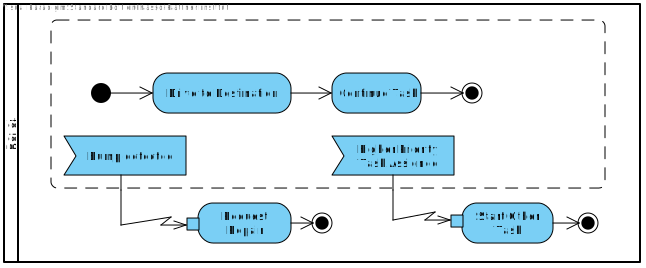
\includegraphics[width=\textwidth]{img/TakeCustomerToDestination}
				\caption{Illustration von \emph{4: Take Customer to Destination} durch Aktivitätendiagramm}
				\label{fig:2-4-take-customer-to-destination-aktivitaetendiagramm}
			\end{figure}
	\pagebreak

	


\section{Produktfunktionen}
	% \input{3-Produktfunktionen}

		\subsection{Use Cases}
		% \input{3-1-Use_Cases}
		
		Die Abbildungen \ref{fig:3-1-robot-use-cases}, \ref{fig:3-1-server-use-cases} und \ref{fig:3-1-hospital-use-cases} zeigen die Funktionalitäten der Teilsysteme \emph{Robot}, \emph{Server} sowie \emph{Hospital}.
		
			\begin{figure}[H]
				\centering
				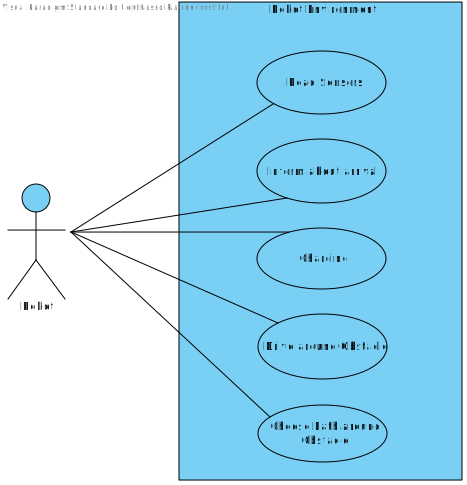
\includegraphics[width=0.8\textwidth]{img/1-Analyse-3-Robot}
				\caption{Use Case Diagramm 1: Use Cases des Robots}
				\label{fig:3-1-robot-use-cases}
			\end{figure}

			\begin{figure}[H]
				\centering
				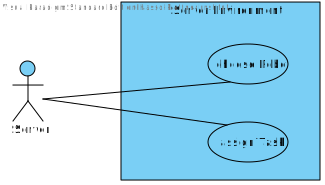
\includegraphics[width=0.8\textwidth]{img/1-Analyse-3-Server}
				\caption{Use Case Diagramm 2: Use Cases des Servers}
				\label{fig:3-1-server-use-cases}
			\end{figure}

			\begin{figure}[H]
				\centering
				\includegraphics[width=0.8\textwidth]{img/1-Analyse-3-Hospital}
				\caption{Use Case Diagramm 2: Use Cases des Hospitals}
				\label{fig:3-1-hospital-use-cases}
			\end{figure}

		\pagebreak

		\subsection{Beschreibung zu Use Case \emph{1}: Choose Path around Obstacle}

			\subsubsection*{Charakterisierende Informationen}

			\begin{table}[H]
				\centering
				\begin{tabularx}{\textwidth}{@{}p{5cm}X@{}}
				\hline
				\textbf{Übergeordneter elementarer Geschäftsprozess:} & Drive to Destination\\ \hline
				\textbf{Ziel des Use Cases:} & \emph{Robot} wählt einen Weg um ein \emph{Obstacle} \\ \hline
				\textbf{Umgebende Systemgrenze:} & \emph{Robot} \\ \hline
				\textbf{Vorbedingung:} & Der \emph{Robot} befindet sich dabei, eine \emph{Destination} anzufahren \\ \hline
				\textbf{Nachbedingung bei erfolgreicher Ausführung:} & 
				Der \emph{Robot} umfährt das \emph{Obstacle} \\ \hline
				\textbf{Beteiligte Nutzer:} & \emph{Robot} \\ \hline
				\textbf{Auslösendes Ereignis:} & Ein \emph{Robot} hat ein \emph{Obstacle} auf dem Weg zwischen sich und der \emph{Destination} gefunden\\ \hline
				\end{tabularx}
			\end{table}

			Dieser Use Case wird dann benutzt, wenn ein \emph{Robot} auf dem Weg zu seiner aktuellen \emph{Destination} ein \emph{Obstacle} vor sich findet, das umfahren werden muss. Im Wesentlichen spricht der Robot dann seine Peripherie an, um Informationen über das \emph{Obstacle} zu sammeln. Dabei findet eine Fallunterscheidung statt, sodass sich zum Beispiel zwei gegenüberstehende \emph{Robots} erkennen und beide nach rechts ausweichen. Bei statischen \emph{Obstacles} wird diese Entscheidung abhängig von dem Teil des \emph{Obstacles} entschieden, den der \emph{Robot} mit seinen Sensoren wahrnehmen kann.
		
		\pagebreak
		
		
		\subsection{Beschreibung zu Use Case \emph{2}: Drive around Obstacle}

			\subsubsection*{Charakterisierende Informationen}

			\begin{table}[H]
				\centering
				\begin{tabularx}{\textwidth}{@{}p{5cm}X@{}}
				\hline
				\textbf{Übergeordneter elementarer Geschäftsprozess:} & Drive to Destination\\ \hline
				\textbf{Ziel des Use Cases:} & \emph{Robot} umfährt ein \emph{Obstacle} \\ \hline
				\textbf{Umgebende Systemgrenze:} & \emph{Robot} \\ \hline
				\textbf{Vorbedingung:} & Ein \emph{Robot} hat ein \emph{Obstacle} auf dem Weg zwischen sich und der \emph{Destination} gefunden\\ \hline
				\textbf{Nachbedingung bei erfolgreicher Ausführung:} & 
				Der \emph{Robot} umfährt das \emph{Obstacle} \\ \hline
				\textbf{Beteiligte Nutzer:} & \emph{Robot} \\ \hline
				\textbf{Auslösendes Ereignis:} & Der \emph{Robot} hat den besten (nach seinen Berechnungen) Weg um das \emph{Obstacle} gewählt. \\ \hline
				\end{tabularx}
			\end{table}
		Dieser Use Case beschreibt die eigentliche Umfahrung eines \emph{Obstacles} von einem \emph{Robot}. Der \emph{Robot} hat davor ausgewählt, zu welcher Richtung hin er das \emph{Obstacle} umfahren möchte. Wenn es sich um ein statisches \emph{Obstacle} handelt, fährt der \emph{Robot} immer eine kleine Distanz parallel zur Kante des \emph{Obstacles} und prüft ob der Weg zur \emph{Destination} wieder frei ist. Wenn dieser frei ist, wird die normale Fahrt wieder aufgenommen, ansonsten wird der Kurs wieder parallel zur Kante des \emph{Obstacles} korrigiert und der Vorgang wiederholt. Wenn sich zwei \emph{Robots} gegenseitig als \emph{Obstacles} wahrgenommen haben, ist ihnen aus dem Use Case \textit{Choose Path around Obstacle} klar, dass sie beide nach rechts ausweichen müssen, um dann den Normalbetrieb wieder aufzunehmen.
			
			%\subsubsection*{Beschreibung des allgemeinen Ablaufes}
			
		\pagebreak

		\subsection{Beschreibung zu Use Case \emph{3}: Read Sensors}

			\subsubsection*{Charakterisierende Informationen}

			\begin{table}[H]
				\centering
				\begin{tabularx}{\textwidth}{@{}p{5cm}X@{}}
				\hline
				\textbf{Übergeordneter elementarer Geschäftsprozess:} & Choose Robot\\ \hline
				\textbf{Ziel des Use Cases:} & \emph{Robot} kann über seinen Akkustand und seine Position Auskunft geben\\ \hline
				\textbf{Umgebende Systemgrenze:} & \emph{Robot} \\ \hline
				\textbf{Vorbedingung:} & \emph{Robot} hat eine Anfrage vom \emph{Server} erhalten \\ \hline
				\textbf{Nachbedingung bei erfolgreicher Ausführung:} & \emph{Robot} schickt die ermittelten Informationen an den \emph{Server} \\ \hline
				\textbf{Beteiligte Nutzer:} & \emph{Robot} \\ \hline
				\textbf{Auslösendes Ereignis:} & \emph{Robot} hat eine Anfrage vom \emph{Server} erhalten, seine Sensoren zu lesen und sie dem \emph{Server} zu schicken \\
				\hline
				\end{tabularx}
			\end{table}

			Im Rahmen vom Geschäftsprozess \emph{Choose Robot} sammelt der \emph{Server}
			Informationen über jeden \emph{Robot}. Diese Informationen (z.B
			Akkustand, aktuelle Position, ob der \emph{Robot} gerade ein Ziel verfolgt)
			kann der \emph{Robot} von seinen Hardware-Schnittstellen anfordern. Dieses
			Use Case wird dann ausgefüht, wenn der \emph{Robot} eine Anfrage vom
			Server erhält, seine Sensoren zu lesen, und endet damit, dass der \emph{Robot}
			die zusammengefassten Informationen an den \emph{Server} schickt.

			\subsubsection*{Szenario für den Standardablauf (Erfolg)}

			\begin{table}[H]
				\centering
				\begin{tabularx}{\textwidth}{@{}cp{2cm}X@{}}
				\hline
				Schritt & Nutzer & Beschreibung der Aktivität \\ \hline
				1 & Robot & \emph{Robot} erhält Anfrage vom \emph{Server} \\
				2 & Robot & \emph{Robot} sammelt Informationen von seiner Hardwareschnittstelle und fasst sie zusammen \\
				3 & Robot & \emph{Robot} schickt zusammengefasste Informationen an den Server \\
				\hline
				\end{tabularx}
			\end{table}

			%\subsubsection*{Beschreibung des allgemeinen Ablaufes}
			
		\pagebreak

		\subsection{Beschreibung zu Use Case \emph{4}: Charging}

			\subsubsection*{Charakterisierende Informationen}

			\begin{table}[H]
				\centering
				\begin{tabularx}{\textwidth}{@{}p{5cm}X@{}}
				\hline
				\textbf{Übergeordneter elementarer Geschäftsprozess:} & Drive to Destination\\ \hline
				\textbf{Ziel des Use Cases:} & Ziel ist es, dem \emph{Robot} zu ermöglichen seine Ladestation anzufahren\\ \hline
				\textbf{Umgebende Systemgrenze:} & \emph{Robot}\\ \hline
				\textbf{Vorbedingung:} & Der \emph{Robot} erreicht sein vorgegebenes Ziel\\ \hline
				\textbf{Nachbedingung bei erfolgreicher Ausführung:} & Der \emph{Robot} erreicht seine Ladestation\\ \hline
				\textbf{Beteiligte Nutzer:} & \emph{Robot}\\ \hline
				\textbf{Auslösendes Ereignis:} & \emph{Robot} erreicht \emph{Destination} (Use-Case)\\
				\hline
				\end{tabularx}
			\end{table}

			Jedem Robot wird, laut Aufgabenstellung, eine feste Ladestation zugewiesen. Der Robot fährt vollständig autonom diese Ladestation an. Daher ist keine Kommunikation mit dem Server notwendig.

			\subsubsection*{Szenario für den Standardablauf (Erfolg)}

			\begin{table}[H]
				\centering
				\begin{tabularx}{\textwidth}{@{}cp{2cm}X@{}}
				\hline
				Schritt & Nutzer & Beschreibung der Aktivität \\ \hline
				1 & Robot & \emph{Robot} erreicht Ziel \\
				2 & Robot & \emph{Robot} fährt zur Ladestation \\
				3 & Robot & \emph{Robot} erreicht Ladestation und lädt sich auf \\
				4 & Robot & \emph{Robot} erhält neues Ziel und fährt dorthin \\
				\hline
				\end{tabularx}
			\end{table}

			%\subsubsection*{Beschreibung des allgemeinen Ablaufes}
			
		\pagebreak
		
			\subsection{Beschreibung zu Use Case \emph{5}: Inform about arrival}

			\subsubsection*{Charakterisierende Informationen}

			\begin{table}[H]
				\centering
				\begin{tabularx}{\textwidth}{@{}p{5cm}X@{}}
				\hline
				\textbf{Übergeordneter elementarer Geschäftsprozess:} & TakePatientToHospital\\ \hline
				\textbf{Ziel des Use Cases:} & Ziel ist es, dem \emph{Robot} zu ermöglichen seine Ankunft dem Krnakenhaus mitzuteilen\\ \hline
				\textbf{Umgebende Systemgrenze:} & \emph{Robot}\\ \hline
				\textbf{Vorbedingung:} & Der \emph{Robot} erreicht die \emph{Position} des Patienten\\ \hline
				\textbf{Nachbedingung bei erfolgreicher Ausführung:} & Der \emph{Robot} wartet, bis er beladen wurde\\ \hline
				\textbf{Beteiligte Nutzer:} & \emph{Robot}\\ \hline
				\textbf{Auslösendes Ereignis:} & \emph{Robot} erreicht Patienten\\
				\hline
				\end{tabularx}
			\end{table}

			Der \emph{Robot} erreicht seine vorgegebene \emph{Destination} und muss dem \emph{Hospital} mitteilen, dass er angekommen ist. 

			\subsubsection*{Szenario für den Standardablauf (Erfolg)}

			\begin{table}[H]
				\centering
				\begin{tabularx}{\textwidth}{@{}cp{2cm}X@{}}
				\hline
				Schritt & Nutzer & Beschreibung der Aktivität \\ \hline
				1 & Robot & \emph{Robot} informiert \emph{Server}, dass er angekommen ist. \\
				\hline
				\end{tabularx}
			\end{table}

			%\subsubsection*{Beschreibung des allgemeinen Ablaufes}
			
		\pagebreak

		\subsection{Beschreibung zu Use Case \emph{6}: Select best Match}

			\subsubsection*{Charakterisierende Informationen}

			\begin{table}[H]
				\centering
				\begin{tabularx}{\textwidth}{@{}p{5cm}X@{}}
				\hline
				\textbf{Übergeordneter elementarer Geschäftsprozess:} & Choose Robot \\ \hline
				\textbf{Ziel des Use Cases:} & Passenden \emph{Robot} für die aktuelle \emph{Destination} auswählen\\ \hline
				\textbf{Umgebende Systemgrenze:} & \emph{Robot} und \emph{Server} \\ \hline
				\textbf{Vorbedingung:} & \emph{Server} sucht \emph{Robot} für eine neu erhaltene \emph{Destination}\\ \hline
				\textbf{Nachbedingung bei erfolgreicher Ausführung:} & Wenn es einen geeigneten \emph{Robot} gibt, dann wird diesem die \emph{Destination} zugeteilt.\\ \hline
				\textbf{Beteiligte Nutzer:} & \emph{Robot} und \emph{Server}\\ \hline
				\textbf{Auslösendes Ereignis:} & \emph{Server} hat von allen \emph{Robots} die Sensordaten empfangen\\
				\hline
				\end{tabularx}
			\end{table}

			\subsubsection*{Szenario für den Standardablauf (Erfolg)}

			\begin{table}[H]
				\centering
				\begin{tabularx}{\textwidth}{@{}cp{2cm}X@{}}
				\hline
				Schritt & Nutzer & Beschreibung der Aktivität \\ \hline
				1 & Server & \emph{Server} erhält Sensordaten von allen \emph{Robots} \\
				2 & Server & \emph{Server} berechnet, ob es einen \emph{Robot} gibt, der zur \emph{Destination} fahren kann\\
				3 & Server & Wenn es keinen geeigneten \emph{Robot} gibt, weise die \emph{Destination} ab. \\
				4 & Server & Es gitb einen geeigneten \emph{Robot} und \emph{Server} führt den Use-Case \textit{Assign Task} aus und gibt dem \emph{Robot} die \emph{Destination}\\
				\hline
				\end{tabularx}
			\end{table}

			%\subsubsection*{Beschreibung des allgemeinen Ablaufes}
			
		\pagebreak

		\subsection{Beschreibung zu Use Case \emph{7}: Assign Task}

			\subsubsection*{Charakterisierende Informationen}

			\begin{table}[H]
				\centering
				\begin{tabularx}{\textwidth}{@{}p{5cm}X@{}}
				\hline
				\textbf{Übergeordneter elementarer Geschäftsprozess:} & Choose Robot  \\ \hline
				\textbf{Ziel des Use Cases:} & \emph{Robot} den Task (die \emph{Destination}) zuweisen\\ \hline
				\textbf{Umgebende Systemgrenze:} & \emph{Server} und \emph{Robot} \\ \hline
				\textbf{Vorbedingung:} & „Choose Robot“ hat den am besten geeigneten \emph{Robot} gefunden und ausgewählt\\ \hline
				\textbf{Nachbedingung bei erfolgreicher Ausführung:} & Ausgewählter \emph{Robot} steuert die \emph{Destination} an\\ \hline
				\textbf{Beteiligte Nutzer:} & \emph{Server} und \emph{Robot}\\ \hline
				\textbf{Auslösendes Ereignis:} & Im Use-Case „choose Robot“ wurde passender \emph{Robot} ausgewählt\\
				\hline
				\end{tabularx}
			\end{table}
			
			Dem \emph{Server} wird hiermit die Möglichkeit gegeben, dem \emph{Robot} eine beliebige \emph{Destination} zuzuweisen. 

			\subsubsection*{Szenario für den Standardablauf (Erfolg)}

			\begin{table}[H]
				\centering
				\begin{tabularx}{\textwidth}{@{}cp{2cm}X@{}}
				\hline
				Schritt & Nutzer & Beschreibung der Aktivität \\ \hline
				1 & Server & \emph{Server} überträgt ausgewähltem \emph{Robot} den Task \\
				\hline
				\end{tabularx}
			\end{table}

			%\subsubsection*{Beschreibung des allgemeinen Ablaufes}

	\pagebreak


		\subsection{Beschreibung zu Use Case \emph{8}: Check availability}

			\subsubsection*{Charakterisierende Informationen}

			\begin{table}[H]
				\centering
				\begin{tabularx}{\textwidth}{@{}p{5cm}X@{}}
				\hline
				\textbf{Übergeordneter elementarer Geschäftsprozess:} & TakePatientToHospital  \\ \hline
				\textbf{Ziel des Use Cases:} & \emph{Hospital} erfährt, ob ein Auftrag vom System entgegengenommen werden kann. \\ \hline
				\textbf{Umgebende Systemgrenze:} & \emph{Hospital} und \emph{Server} \\ \hline
				\textbf{Vorbedingung:} & Das \emph{Hospital} hat einen neuen Patienten registriert. \\ \hline
				\textbf{Nachbedingung bei erfolgreicher Ausführung:} & Das System führt den Auftrag aus und bringt den \emph{Patient} in das \emph{Hospital} \\ \hline
				\textbf{Beteiligte Nutzer:} & \emph{Hospital} und \emph{Server}\\ \hline
				\textbf{Auslösendes Ereignis:} & \emph{Hospital} hat einen neuen Auftrag\\
				\hline
				\end{tabularx}
			\end{table}

			Das \emph{Hospital} fragt laut Aufgabenstellung an dem zu modellierenden System an, ob ein \emph{Robot} verfügbar ist, um einen \emph{Patient} anzufahren und ins \emph{Hospital} zu bringen. Dazu wird vom \emph{Server} unter anderem der Use Case \emph{Choose Robot} ausgeführt. Es kann passieren, dass kein \emph{Robot} verfügbar ist, dann soll wie in der Aufgabenstellung beschrieben der Auftrag vom System abgelehnt werden. Was das \emph{Hospital} dann für Maßnahmen ergreift, wird hier nicht modelliert da es nicht teil des Systems ist.

			%\subsubsection*{Beschreibung des allgemeinen Ablaufes}

	\pagebreak
		\subsection{Beschreibung zu Use Case \emph{9}: Inform about boarding}

			\subsubsection*{Charakterisierende Informationen}

			\begin{table}[H]
				\centering
				\begin{tabularx}{\textwidth}{@{}p{5cm}X@{}}
				\hline
				\textbf{Übergeordneter elementarer Geschäftsprozess:} & TakePatientToHospital   \\ \hline
				\textbf{Ziel des Use Cases:} & Dem \emph{Robot} mitteilen, dass Patient auf den \emph{Robot} beladen wurde \\ \hline
				\textbf{Umgebende Systemgrenze:} & \emph{Hospital} \\ \hline
				\textbf{Vorbedingung:} & Patient befindet sich auf \emph{Robot}\\ \hline
				\textbf{Nachbedingung bei erfolgreicher Ausführung:} & \emph{Robot} fährt Patienten zum \emph{Hospital} \\ \hline
				\textbf{Beteiligte Nutzer:} & \emph{Hospital}\\ \hline
				\textbf{Auslösendes Ereignis:} & \emph{Server} wurde informiert, dass \emph{Robot} am Patienten angekommen ist(Inform about arrival)\\
				\hline
				\end{tabularx}
			\end{table}
			
			Das \emph{Hospital} muss dem \emph{Robot} mitteilen, dass der Patient beladen wurde um einen sicheren Transport des Patienten zu gewährleisten. Der \emph{Robot} hat somit keinen Eingriff in das Beladen des Patienten.

			\subsubsection*{Szenario für den Standardablauf (Erfolg)}

			\begin{table}[H]
				\centering
				\begin{tabularx}{\textwidth}{@{}cp{2cm}X@{}}
				\hline
				Schritt & Nutzer & Beschreibung der Aktivität \\ \hline
				1 & \emph{Hospital} & Patient wird auf Roboter beladen \\
				2 & \emph{Hospital} & \emph{Hospital} sendet Nachricht an Server, dass sich Patient auf dem \emph{Robot} befindet \\
				\hline
				\end{tabularx}
			\end{table}

			%\subsubsection*{Beschreibung des allgemeinen Ablaufes}

	\pagebreak


\section{Produktumgebung}

  \subsection{Systemumgebung}
  Im nachfolgenden Abschnitt werden die bekannten Komponenten des Systems und die dazugehörigen Schnittstellen beschrieben.
  Grundsätzlich besteht das System aus mindestens einer \emph{RobotUnit}, hierfür geeigneten \emph{Chargern} und einem zentralen \emph{Server}, über welchen das \emph{Hospital} und die \emph{Taxi Customer} mithilfe der \emph{TaxiApp} mit dem System interagieren können.

  \subsubsection{Hardwareumgebung}

    \paragraph{Server}\label{server}

    Es existiert ein zentraler \emph{Server}, der über ausreichende Ressourcen verfügt.
    Dieser \emph{Server} besitzt einen zentralen Hauptprozessor, den \emph{ServerCore}, über den er auf alle weiteren Komponenten zugreifen kann.
    Zu diesen Komponenten zählt der \emph{WlanAdapter}, über welchen der \emph{Server} auf das Funknetzwerk zugreifen kann.
    Über dieses Funknetzwerk können alle \emph{RobotUnits} erreicht werden, sodass Nachrichten an sie abgesetzt werden können und Nachrichten, die über das Funknetzwerk für den \emph{Server} übertragen wurden, empfangen werden können.
    Über eine weitere Komponente, den \emph{HospitalAdapter}, kann der \emph{Server} mit dem zentralen \emph{Hospital} kommunizieren.
    Die Kommunikation mit den \emph{Taxi-Customers} wird ebenfalls über die gesonderte Komponente \emph{TaxiAppAdapter} mit ähnlicher Funktionalität realisiert.

    \paragraph{RobotUnit}\label{robotunit}

    Das Transportvehikel \emph{RobotUnit} stellt die Kernkomponente der Hardwareumgebung dar.
    Über den zentralen Hauptprozessor \emph{RobotCore} kann auf alle weiteren Komponenten zugegriffen werden.
    Als Antrieb nutzt das Transportvehikel die \emph{RobotEngine}: einen omnidirektionalen Antrieb mit 3 Motoren, über welchen es sich vorwärts, nach rechts, nach links oder durch Drehen um die eigene Achse bewegen lässt.
    Der Antrieb ermöglicht eine Fahrt in verschiedenen Geschwindigkeiten.
    Die \emph{RobotUnit} verfügt außerdem über die Komponente \emph{DistanceSensor} bestehend aus 9 Infarotdistanzsensoren, die an der kreisförmigen Außenwand des Vehikels im Abstand von jeweils 40 Grad angeordnet sind.
    Über sie ist die Feststellung der Entfernung des Vehikels von allen bewegten und unbewegten Objekten in der Umgebung möglich.
    Bei einer Kollision der \emph{RobotUnit} mit einem anderen Objekt wird dieses Ereignis über die Sensorik der Kollisionserkennung \emph{Bumper} festgestellt, woraufhin der \emph{Robot} über den \emph{Server} die Reparatur durch einen externen Anbieter anfordert.
    Über das GPS-Modul \emph{NorthStar} kann die aktuelle Lage und Ausrichtung der \emph{RobotUnit} ermittelt werden.
    Zur Ermöglichung von Kommunikation besitzt die \emph{RobotUnit} einen \emph{WlanAdapter}, über welchen Nachrichten über ein zur Verfügung stehendendes Funknetzwerk gesendet und empfangen werden können.
    Jede \emph{RobotUnit} verfügt über einen Akkumulator \emph{Battery}, der zur Energieversorgung dient.
    Eine ausreichende Ladung des Akkumulators ist zum Betrieb der \emph{RobotUnit} unbedingt erforderlich.
    Der Akkumulator kann über einen \emph{Charger} geladen werden.

    \paragraph{Charger}\label{charger}

    Es existieren die Ladestationen \emph{Charger}, über die sich die \emph{Battery} der \emph{RobotUnit} vollständig laden lässt.
    Eine Ladestation ist dabei genau einer \emph{RobotUnit} zugeordnet.
    Zum Laden muss eine \emph{RobotUnit} seine Ladestation anfahren, worauf die Ladung sofort beginnt.
    Jede Ladestation verfügt über eine feste Position.

    \paragraph{Hospital}\label{hospital}

    Es existiert außerdem ein zentrales Krankenhaus, das \emph{Hospital}.
    Das \emph{Hospital} befindet sich an einer festen Position, die die \emph{RobotUnits} anfahren können, um \emph{Patients} dem Personal zu übergeben.
    Über die \emph{Hospital}-Komponente des Servers kann das \emph{HospitalAdapter} auf nicht näher spezifizierte Weise mit dem Server kommunizieren.

  \subsubsection{Softwareumgebung}

    \paragraph{Server}\label{server}
    		Auf dem \emph{Server} läuft, da nicht anders angegeben, ein Standard-Betriebssystem.
    		Darauf läuft eine Laufzeitumgebung, die die benötigten Methoden zur Kommunikation mit den \emph{RobotUnits} bereitstellt.
    	\subparagraph{NetworkAccess}\label{networkaccess}
    		Der \emph{NetworkAccess} ist die Schnittstelle des \emph{Servers}, mit der er die Verbindung zu den \emph{RobotUnits} herstellt.
        Hierüber werden Nachrichten ausgetauscht.
    		Dementsprechend stehen Methoden zum Senden einer Message, Registrieren eines IMessageHandlers, Auslesen von NetworkIDs usw. bereit.
    	\subparagraph{HospitalAdapter}\label{hospital}
    		Bei \emph{HospitalAdapter} handelt es sich um die \emph{Server}-Komponente, die die Kommunikation mit dem \emph{Hospital} gewährleistet.
    		Dabei werden zum einen Methoden bereitgestellt, die das \emph{Hospital} über ein Interface aufrufen kann, um Aufträge zu verteilen und dem \emph{Hospital} Informationen über den aktuellen Stand des Auftrags mitzuteilen (getPatientAt(), patientOnBoard() sowie patientArrived()), und zum anderen kann die Komponente über ein Interface Methoden des \emph{Hospitals} aufrufen, um diesem Informationen zu übermitteln (informRobotArrivedAtPatient() und informRobotArrivedAtHospital()).
      \subparagraph{TaxiApp}
        Die \emph{TaxiApp}-Komponente ist ein Container, über den die Kommunikation des \emph{Servers} mit den Apps der \emph{Taxi Customers}, den nicht-modellierten mobilen Taxi-Applikationen, realisiert wird.
        Der Container stellt ein Taxi-App Objekt für jeden Benutzer bereit.
        Die Kommunikation findet über mehrere Schnittstellen statt.
        Über das \emph{IAppContainer}-Interface kann der \emph{Server} Taxi-App Objekte bekommen.
        Über die Interfaces \emph{ITaxiAppUserOutput} und \emph{ITaxiAppUserInputHandler} kann der \emph{Server} mit den einzelnen Apps und damit mit den \emph{Taxi-Customers} kommunizieren.
        Das \emph{ITaxiApp}-Interface stellt die Methoden zum Zugriff aud die Kommunikationsinterfaces, sowie eine Methode zur Ermittlung der App-ID bereit.
    \paragraph{RobotUnit}\label{robotunit}
    		Nachfolgend werden die zentralen Softwareschnittstellen der \emph{RobotUnit} beschrieben.
    	\subparagraph{RobotCore}\label{robotcore}
    		Auf der zentralen Recheneinheit der \emph{RobotUnit}, dem \emph{RobotCore}, läuft eine JavaRuntimeEnvironment, in der sich die gesamte Steuerung und die Verwendung der Komponenten und Schnittstellen abspielt.
    		Die einzelnen Komponenten mit ihren Methoden werden im Folgenden näher erläutert.
    	\subparagraph{IRSensorDistance}\label{irsensordistance}
    		Die \emph{IRSensorDistance}-Schnittstelle stellt drei Methoden bereit, mit denen die Distanz und der Winkel des entdeckten Objekts und der an der Entdeckung beteiligte Infrarotsensor erfasst und in Arrays gespeichert werden.
    	\subparagraph{IDistanceSensor}\label{idistancesensor}
    		Die besagten Arrays kann der \emph{IDistanceSensor} auslesen.
    		Er hat dazu ebenfalls drei Methoden: getIRDistances() gibt ein Array mit allen erfassten Objekten zurück, getIRDistancesInRange() gibt ebenfalls ein Array zurück, das allerdings nur die Objekte in einem gewissen Abstand enthält und getNearestIRDistances() gibt nur das nächste Objekt zurück.
    	\subparagraph{INorthStar}\label{inorthstar}
    		Die Schnittstelle \emph{INorthStar} ist für die Bestimmung der Positionierung zuständig und greift dabei auf ein Device zur Standortbestimmung zurück.
    		Sie hat zwei Methoden.
    		Eine liest die aktuelle Position aus, die Andere die aktuelle Ausrichtung.
    		Die Position besteht dabei aus zwei float-Werten, einer x- und einer y-Koordinate.
    	\subparagraph{IWlanAdapter}\label{iwlanadapter}
    		Bei \emph{IWlanAdapter} handelt es sich um die Schnittstelle, mit der auf Seite der \emph{RobotUnit} die Kommunikation zwischen \emph{RobotUnit} und \emph{Server} ermöglicht wird.
    		Entsprechend gibt es hier die gleichen Methoden zur Kommunikation, die auch die \emph{IWlanAdapter}-Schnittstelle des \emph{Servers} bereitstellt.
    	\subparagraph{IBumperHandler}\label{ibumperhandler}
    		\emph{IBumperHandler} ist das Interface zum Umgang mit Zusammenstößen.
    		Die Kollisionserkennung registriert über \emph{IBumper} einen Aufprall und das \emph{IBumperHandler}-Interface stellt zwei Methoden zum Umgang mit dem Aufprall bereit.
    	\subparagraph{IDrive}\label{idrive}
    		Die Bewegungssteuerung der \emph{RobotUnit} heißt \emph{IDrive}.
    		Sie stellt vier Methoden bereit.
    		Die Methoden driveToPosition() und driveToPositionCautiously() erwarten beide eine Position, eine Geschwindigkeit und einen ArrivalHandler, der eine Methode zur Meldung aufruft, wenn die \emph{RobotUnit} am Ziel angekommen ist.
    		Beide Methoden dienen dazu, ein gegebenes Ziel anzufahren, wobei bei der Zweiten die Höchstgeschwindigkeit geringer ist.
    		Die Höchstgeschwindigkeit für Cautiously, Regular und Fast Methoden stellt das \emph{IDrive}-Interface bereit, wobei Cautiously $\leq$ Regular $\leq$ Fast gilt.
    		Die anderen beiden Methoden, drive() und driveCautiously() unterscheiden sich ebenfalls nur in der Höchstgeschwindigkeit und ermöglichen ein manuelles Fahren.
    		Dabei erwarten sie die Drehung der \emph{RobotUnit} als float-Wert sowie die Vorwärts- und die Seitwärtsgeschwindigkeit, ebenfalls als float-Wert.
    	\subparagraph{IBattery}\label{ibattery}
    		Bei \emph{IBattery} handelt es sich um die Akkusteuerung der \emph{RobotUnit}.
    		Sie stellt zwei Methoden bereit.
    		getBatteryLevel() gibt den aktuellen Akkuladestand als float-Wert zurück, getChargingPosition() gibt die Position des zugeordneten \emph{Chargers} zurück.


\pagebreak
\subsubsection{Ressourcenübersicht}
    In Abbildung \ref{fig:4-1-3-verteilungsdiagramm} werden die in 4.1.1 und 4.1.2 beschriebenen
    Komponenten und Schnittstellen im Verteilungsdiagramm dargestellt.

    \begin{figure}[H]
      \centering
      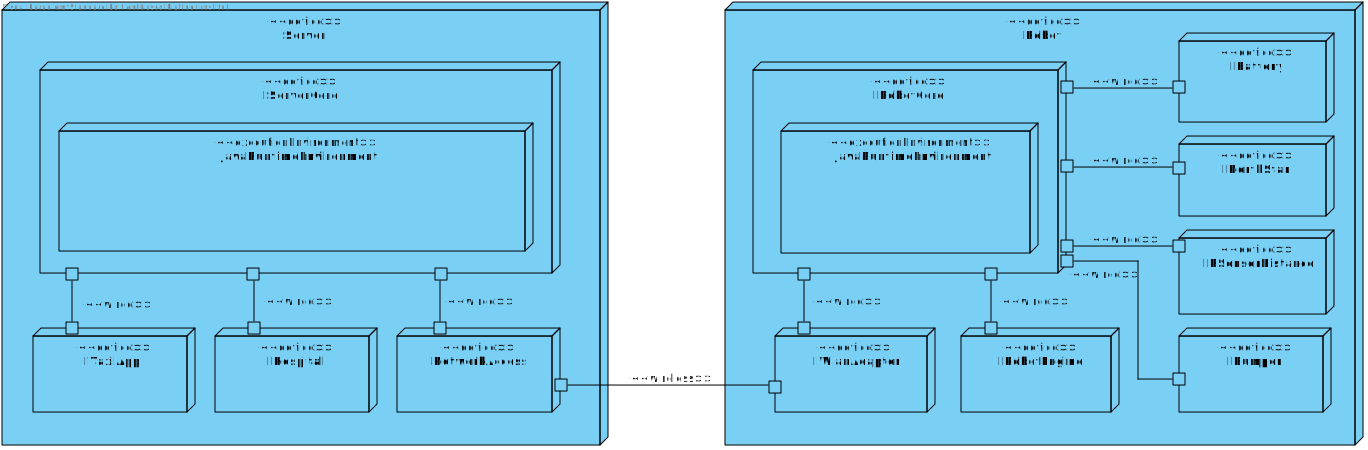
\includegraphics[width=1.25\textwidth, angle=90]{img/2-Analyse-4-Produktumgebung}
      \caption{Verteilungsdiagramm}
      \label{fig:4-1-3-verteilungsdiagramm}
    \end{figure}


\end{document}
